Though the line-integrated metastable densities are one of only a few
measurements made in the development of the \acs{rpnd}, they only provide a
limited view of what is happening. In addition to the metastables are ions,
electrons, a vast array of other excited states, and the electric fields. In an
effort to expand on the details of what is occurring within the \acs{rpnd}, it
is desirable to develop a model which can infer other properties from the
metastable measurements. This is possible, because the electrons which gain
energy from the electric fields are responsible for the excitation of the
metastables, other atomic states, and ions. The ideal model would solve the
Boltzmann equation (equation~\ref{eq:boltzmann}) for each species, over the
entire geometry, in all dimensions, for as long as was required to reach
equilibrium.

Unfortunately, these requirements are somewhat problematic. Solutions to the
Boltzmann equation alone are difficult \cite{Lieberman2005}, let alone for the
dozens of species which may be present in the \acs{rpnd}. The spatial
discretization can be estimated as the cube of the largest length scale (the
discharge apparatus length, about 30 cm) divided by the smallest length scale
(on the order of the Debye length, about 20 $\mu$m). This approximation suggests
the need for $2\times10^{12}$ spatial cells. Similar calculations can be made
for the time (from nanoseconds to minutes) and velocity (from thermal to 100s of
eV) scales. It is immediately apparent that a numerical system of this size
would exceed the capabilities of any existing computer.

\section{Model Development}

Therefore, some approximations of the Boltzmann equation were required in order
to obtain a computationally tractable problem. As discussed in
Chapter~\ref{chp:theory}, the most common approach, and the one applied here, is
the use of \emph{moments} of the Boltzmann equation. These moments average out
the velocity dependence of the Boltzmann equation in favor of macroscopic
properties such as particle densities and mean velocities. They are often used
to develop various fluid approximations for plasmas \cite{Chen1984} (e.g.\ the
two fluid model, the magnetohydrodynamic equations, etc.). Solutions of
these fluid equations have been tremendously successful in the description of
everything from plasma display panels \cite{Rauf1999b} to interstellar plasmas
\cite{Linde1998}.

The use of moments of the Boltzmann equation does introduce some additional
problems. Reaction rates, such as ionization and excitation, are very sensitive
to changes in the distribution of particle velocities. This presents a problem
as the moments of the Boltzmann equation average out the velocity dependence.
Therefore, a distribution function must be assumed or calculated in order to
determine the reaction rates. The Maxwell-Boltzmann and Druyvesteyn
distributions from Chapter~\ref{chp:theory} are often used for this purpose.
However, they require a number of assumptions which are not necessarily true for
most plasmas. In cases when these distributions cannot be applied, approximate
solutions of the Boltzmann equation are often used \cite{Hagelaar2005} which
employ detailed reaction cross sections. The choice between the simple
equilibrium solutions and the more complex approximations is not easy as the
\acs{eedf} is rarely known \emph{a priori}. This topic is considered more
thoroughly in section~\ref{sec:dists}.

From another perspective, fluid models in multiple dimensions are still
computationally expensive. In large geometries, this can limit the number of
species and reactions which can be considered by the simulation
\cite{Lieberman2005}. For this reason, simulations often limit themselves to one
or a few excited states, preventing detailed comparisons to spectroscopic data.
However, such comparisons can reveal information about the degree of equilibrium
in the plasma and the electron temperatures, both of interest in the \acs{rpnd}.
Therefore, additional simplifications were necessary in order include additional
excited states.

As simplifications had already been made to the velocity space, the choice was
between reduced temporal resolution and reduced spatial resolution. A reduction
in temporal resolution was unreasonable given the fixed duration of the pulse
and its afterglow. In contrast, the metastable measurements were already made on
small spatial scale relative to the metastable gradients seen in
Chapter~\ref{chp:metastables}. Therefore, the spatial dependence was eliminated
to produce what is known as a ``global model.'' The final model tracked a total
of 32 different excited states of helium from before the pulse until the return
of the first reflection.

In order to compare the metastable measurements to the global results, it was
necessary to convert the line-integrated densities to densities along the path
of the laser. It has been noted that a similar \acs{fiw} \cite{Vasilyak1994} and
the same \acs{rpnd} \cite{Weatherford2012} exhibit radial variations in emission
intensity, electron density, and metastable density. Unfortunately, the cause of
this is not clearly understood, though it has been suggested that high-energy
electrons from the walls may be responsible \cite{Weatherford2012a}. Lacking any
empirical, theoretical, or numerical results which describe the evolution of the
radial profile during the discharge, it was necessary to assume one. In this
report, the plasma was assumed to be uniform across the diameter of the
discharge. This assumption likely affects the inferred plasma parameters,
however more accurate results are possible provided time-resolved measurements
of the radial metastable density or an improved understanding of the \acs{rpnd}.

\subsection{Continuity Equation}

The equation~\ref{eq:cont}, the continuity equation, forms the basis for
tracking the populations of the excited states in the plasma. Having assumed
that the spatial variations are zero, the equation reduces to,
\begin{equation}
  \frac{d n_\alpha}{dt} = G_\alpha - L_\alpha,
  \label{eq:zdmcont}
\end{equation}
where $\alpha$ identifies the particle species, $G$ is the gain term, and $L$ is
the loss term. The gain and loss terms represent all possible reactions which
can alter the population of the species under consideration. In the presented
model, only helium, excited helium states, helium ions, and electrons were
treated. Also present, to some degree, were gaseous impurities and helium
dimers. As observed in Chapter~\ref{chp:metastables}, the combined effects of
these species on the metastable densities took place with an e-folding time of
about 25 $\mu$s. As the simulations are limited to the period of time before the
first reflection arrives (140 ns), these species were neglected in the model.

There were several possible processes that were considered for inclusion in the
model:
\begin{itemize}
  \singlespacing
  \item electron impact ionization,
  \item electron impact (de)excitation,
  \item atomic impact (de)excitation,
  \item atomic excitation transfer,
  \item dielectronic recombination,
  \item three-body recombination,
  \item radiative decay, and
  \item diffusion.
\end{itemize}
As with the impurities and dimer formation, diffusion occurs on a much longer
time scale, and was subsequently neglected. Three-body recombination in the
volume of the discharge is not important at the estimated temperatures and
densities \cite{Lieberman2005}, therefore this too was neglected. In general,
dielectronic recombination is a rare process \cite{Nahar2010}, however it was
incorporated during early versions and was retained through the final revision.
Inter-atomic excitation and de-excitation is not generally considered important
given the low energies of the atoms in discharges.

The remaining processes were found to be the most important for the \acs{rpnd}.
This included electron-impact ionization and excitation which were, by far, the
most significant. In addition, excitation transfer between atoms was found to
occur at relevant rates \cite{Lieberman2005}. Finally, radiative decay between
states was included as this allowed the prediction of plasma emissions as well
as the cascade of excited states down to the metastable level.

Given these processes, equation~\ref{eq:zdmcont} was rewritten as,
\begin{multline}
  \frac{dN_i}{dt} =   n_e \left[       \sum_{j\neq i} N_j K^e_{j,i}(T_e) 
                                 - N_i \sum_{j\neq i}     K^e_{i,j}(T_e) \right]
                        + \left[       \sum_{j > i}   N_j K^o_{j,i} 
                                 - N_i \sum_{j < i}       K^o_{i,j}      \right] \\
                    + N_g \left[       \sum_{j\neq i} N_j K^a_{j,i} 
                                 - N_i \sum_{j\neq i}     K^a_{i,j}      \right].
  \label{eq:gcont}
\end{multline}
Here, the subscripts of $i$ and $j$ represent states of helium, $N$ is the state
density, $K$ is a rate coefficient, $T_e$ is the electron temperature, and $N_g$
is the neutral helium density. The first subscript of the rate coefficients
represents the initial excited state while the second coefficient represents the
final excited state. Therefore, $K_{ij}$ represents a process that transfers an 
atom from state $i$ to state $j$.

This equation is split into three sets of processes, represented by the
superscripts of the rate coefficients: $e$ - electron impact processes, $o$ -
radiative decay, and $a$ - atomic excitation transfer. The first bracketed term
on the right hand side contains all the rate coefficients for electron impact
excitation and de-excitation, including ionization processes. The second
bracketed term contains the rate coefficients for optical transitions in and out
of the excited state. The final bracketed term contains the gains and losses as
a result of excitation transfer caused by collisions with the ground state.
Collisions between excited states are neglected as their low densities result in
small reaction rates.

The rate coefficients in equation~\ref{eq:gcont} are compiled from a number of
different sources. This is particularly straight forward in the case of the
optical and atomic transitions, as neither features any dependence on the
\acs{eedf}. The optical transition rates and the energies of each level were
obtained from the NIST Atomic Spectra Database \cite{Kramida2012}. The
excitation transfer rate coefficients came from the studies of Catherinot and
Dubreuil \cite{Catherinot1981, Dubreuil1980}. These coefficients only covered
the transitions of $\Delta n=0$ for $n=3,4$ and no constants were found for
other $n$ or $\Delta n\neq 0$. Dielectronic recombination rates were adapted
from the work of Nahar \cite{Nahar2010}.

As for the electron-impact processes, the semi-empirical relations derived by
Ralchenko et al. \cite{Ralchenko2008} were used to calculate the electron
(de)excitation and ionization cross sections for levels through $n=4$. These
represented the most accurate set of cross sections available for neutral helium
and have a quoted accuracy of 10-30\% for $\Delta S=0$, and $>30$\% for $\Delta
S \neq 0$. Only the inelastic cross sections for collisions which increased the
energy of the excited state were provided. The inverse or superelastic cross
sections were calculated using the principle of detailed balance
\cite{Kunze2009},
\begin{equation}
  \sigma_{ji}(\epsilon) = \frac{\epsilon}{\epsilon - \Delta\epsilon_{ij}}
    \frac{g_j^2}{g_i}\sigma_{ij},
\end{equation}
where $\Delta\epsilon$ is the threshold energy of the $ij$ reaction and $g$ is
the statistical degeneracy of the corresponding state. These cross sections can
be used to calculate the rate coefficients for each reaction using
equation~\ref{eq:rate}. However, this leads back to the question of which
\acs{eedf} is appropriate for the \acs{rpnd}.

\subsection{Distribution Effects}\label{sec:dists}

Per the discussion of the Boltzmann equation in Chapter~\ref{chp:theory}, there
are two analytic equilibrium solutions: the Maxwell-Boltzmann distribution, and
the Druyvesteyn distribution. However, research by Starikovskaia and
Starikovskii \cite{Starikovskaia2001} has shown that the \acs{eedf} in a
nitrogen \acs{fiw} can deviate from both. Such a result is not too surprising
given the non-equilibrium nature of the \acs{fiw} discharge. Since the
\acs{rpnd} shares many of these same properties, it is possible that the
equilibrium solutions do not apply to the \acs{rpnd} either.

In order to better understand how the energy distributions may behave in a
\acs{rpnd}, a numerical study of the \acs{eedf} in a helium \acs{rpnd} was
conducted. First, a particle-in-cell (\acs{pic}) code was used to simulate the
effect of a voltage pulse on electrons in a quasi zero-dimensional geometry.
This generated the evolution of the \acs{eedf} in a helium plasma as a function
of time. Then, the mean energy for the \acs{eedf} at each time was calculated.
This was then used to generate similar equivalent Maxwell-Boltzmann
distributions and solutions of the Boltzmann equation.

The \acs{pic} simulations do not attempt to solve the Boltzmann equation
directly. Instead, they simulate the behavior of many plasma particles in an
experimental geometry using the basic laws of motion and electromagnetism
\cite{Birdsall1991}. A discrete \acs{eedf} can then be calculated from the
particle population (or subset thereof). As the number of simulated particles
increases the discrete \acs{eedf} will approach the continuous \acs{eedf} which
would result from a solution of the Boltzmann equation.

Generally, \acs{pic} simulations do not make a one-to-one correspondence between
computer particles and physical particles--most plasma involve more particles
than can be reasonably simulated. Instead, they consider a population of
macro-particles, each of which possesses some statistical weight
\cite{Birdsall1991}. This weight allows the macro-particle to represent a group
of physical particles. Additionally, the velocity and position of the particles
are continuous within the limits of floating point representation. However, the
electromagnetic fields are discretized. This necessitates a mapping of the
particle-related fields to the discretized coordinates, and the force of the
fields from the discretized coordinates to the particles.

Each \acs{pic} simulation begins with the definition of a system geometry and
any external fields. Additionally, simulations are usually initialized with some
number of macro-particles with a specified temperature. After these
initialization steps have been completed, the physics loop illustrated in
figure~\ref{fig:pic},
\begin{figure}
  \centering
  \setlength{\unitlength}{4.8in}
\begin{picture}(1.0, 0.5)
   \put(0.10, 0.35){\framebox(0.35, 0.10){\parbox{0.35\unitlength}{\footnotesize\centering Integration of equations \\ of motion, moving particles \\ $\vec{F}_i \rightarrow \vec{v}'_i \rightarrow x_i$}}}
   \put(0.45, 0.40){\line( 1,  0){0.10}}
   \put(0.55, 0.35){\framebox(0.35, 0.10){\parbox{0.35\unitlength}{\footnotesize\centering Particle loss/gain \\ at the boundaries \\ (emission, absorption, etc.)}}}
   \put(0.90, 0.40){\line( 1,  0){0.05}}
   \put(0.95, 0.40){\line( 0, -1){0.10}}
   \put(0.70, 0.20){\framebox(0.30, 0.10){\parbox{0.30\unitlength}{\footnotesize\centering Monte Carlo collisions \\ $\vec{v}'_i \rightarrow \vec{v}_i$}}}
   \put(0.95, 0.20){\line( 0, -1){0.10}}
   \put(0.95, 0.10){\line(-1,  0){0.10}}
   \put(0.60, 0.05){\framebox(0.25, 0.10){\parbox{0.25\unitlength}{\footnotesize\centering Weighting \\ $(x,\vec{v})_i \rightarrow (\rho, \vec{J})_j$}}}
   \put(0.60, 0.10){\line(-1,  0){0.20}}
   \put(0.15, 0.05){\framebox(0.25, 0.10){\parbox{0.25\unitlength}{\footnotesize\centering Integration of field \\ equations on grid \\ $(\rho, \vec{J})_j \rightarrow (\vec{E},\vec{B})_j$}}}
   \put(0.15, 0.10){\line(-1, 0){0.10}}
   \put(0.05, 0.10){\line( 0, 1){0.10}}
   \put(0.00, 0.20){\framebox(0.20, 0.10){\parbox{0.20\unitlength}{\footnotesize\centering Weighting \\ $(\vec{E},\vec{B})_j \rightarrow \vec{F}_i$}}}
   \put(0.05, 0.30){\line( 0,  1){0.10}}
   \put(0.05, 0.40){\line( 1,  0){0.05}}
   \put(0.46, 0.22){\Huge $\circlearrowright$}
   \put(0.4725, 0.2275){\footnotesize\centering $\Delta t$}
\end{picture}

  \caption{Schematic description of the \acs{pic} simulation process, adapted
    from \cite{Birdsall1991}.}
  \label{fig:pic}
\end{figure}
begins. The equation in the loop reflect a one-dimensional system, thus each
macro particle possesses only one spatial component, $x$. However, an external
magnetic field can cause motion perpendicular to the simulation domain, thus
each macro-particle possesses a velocity vector, $\vec{v}$, with three
components.

The loop generally begins with an initial field calculation based on the
external fields and those of the particles. This is followed by a particle
``push'' where the Lorentz equation, $\vec{F} = q(\vec{E} +
\vec{v}\times\vec{B})$, is used to calculate a new position for a given time
step, $\Delta t$. Afterward, particles which have moved out of the boundaries of
the system are removed from the simulation. Next, collisions (including
ionization and excitation) are modeled using Monte Carlo techniques
\cite{Birdsall1991}. Finally, the charges of the macro-particles are then
weighted to the spatial grid, and the fields are recalculated, and the next time
step begins.

The XPDP1 code, developed by Verboncoeur et al. \cite{Verboncoeur1993}, was used
for the \acs{pic} simulations. The code was originally designed to simulate a
one-dimensional discharge between two parallel electrodes. However, collection
at these electrodes complicates a study of the \acs{eedf} and does not match the
zero-dimensional nature of the global model. Charged particle collection near
the boundaries induces spatial variations in the \acs{eedf}. Additionally, the
high mobility of electrons often means that they are preferentially collected on
short time scales. This leads to the formation of large regions of positive
space charge which shields the plasma from the applied electric field. In order
to address these issues, the code was modified to use periodic boundary
conditions. Such conditions result in a quasi zero-dimensional simulation,
equivalent to a plasma of infinite extent. This eliminates the issue of spatial
variations in the \acs{eedf} and produces a closer match to the assumptions
underlying the global model.

Previous measurements of the electric field in a similar \acs{fiw} suggested
that the electric field values varied from 0-350 Td \cite{Takashima2011}. Based
on this, it was decided to examine the distribution characteristics from 10-600
Td. This range should be adequate to cover all conditions of the \acs{rpnd} in
question. The field was applied immediately after the simulation began. Though
the real field was expected to have a more gradual rise and fall, this was done
in order to exacerbate any non-equilibrium characteristics of the \acs{eedf}.
The background gas was helium at a pressure of 2.0 Torr. The initial plasma was
assumed to be quasineutral with a density of $1.0\times10^{8}$ cm$^{-3}$ and one
computational particle for every $10^6$ physical particles. Electrons were
initialized with a thermal energy of 2.0 eV, and the helium ions were given an
initial energy of 0.025 eV.

The internal set of cross sections were used. These included: elastic
scattering, excitation, and charge exchange. The cross sections were of a
semi-empirical form which increased linearly with energy to a peak value, after
which, they declined as the logarithm of the energy, divided by the energy
\cite{Verboncoeur1993}. The time domain of the simulation was 10 ns. This period
of time was long enough to observe fast \acs{eedf} dynamics associated with the
impulse electric field. The distributions from the \acs{pic} simulations were
sampled every 0.25 ns. The spatial domain was discretized at 1 $\mu$m intervals
over a total domain of 10 cm. Based on the highest energy electrons in the
system, a time step of $4\times10^{-13}$ s was chosen in order to satisfy the
Courant-Friedrich-Lewy stability condition.

BOLSIG+ was used to obtain the approximate solutions of the Boltzmann equation
\cite{Hagelaar2005}. This is a publicly available computer code which uses the
two-term expansion of the Boltzmann equation to solve for the equilibrium
\acs{eedf} for a given electric field. In this approach, Legendre polynomials
are used to expand the \acs{eedf} into a unperturbed component with a small,
superimposed, perturbation. This assumption, that the distribution is accurately
represented by a small perturbation superimposed on an equilibrium solution,
limits the magnitude of the electric fields which the solver can treat. In the
case of the BOLSIG+ calculations for helium, solutions fail to converge for
fields approaching 1000 Td.

The solver was initialized with the cross sections for helium generated by Alves
and Ferreira \cite{Alves2013}. The temporal growth model for electrons was used,
and the electron-electron collisions were neglected as a result of the low
ionization fraction in the \acs{rpnd} (about 10$^{-5}$). Solutions were
calculated for mean energies covering the range of those determined from the
\acs{pic} simulations, from 2-50 eV. The \acs{eedf}s for these solutions were
then tabulated according to their mean energy. A cubic, nearest-neighbor
interpolation scheme was then used to generate an approximate \acs{eedf} for the
precise mean energies from the \acs{pic} simulations.

These same mean energies were used to determine equivalent Maxwell-Boltzmann
distributions for comparison. The \acs{eedf}s generated by the \acs{pic}
simulations, approximate Boltzmann solutions, and Maxwell-Boltzmann
distributions can be seen in figure~\ref{fig:picmb},
\begin{figure}
  \centering
  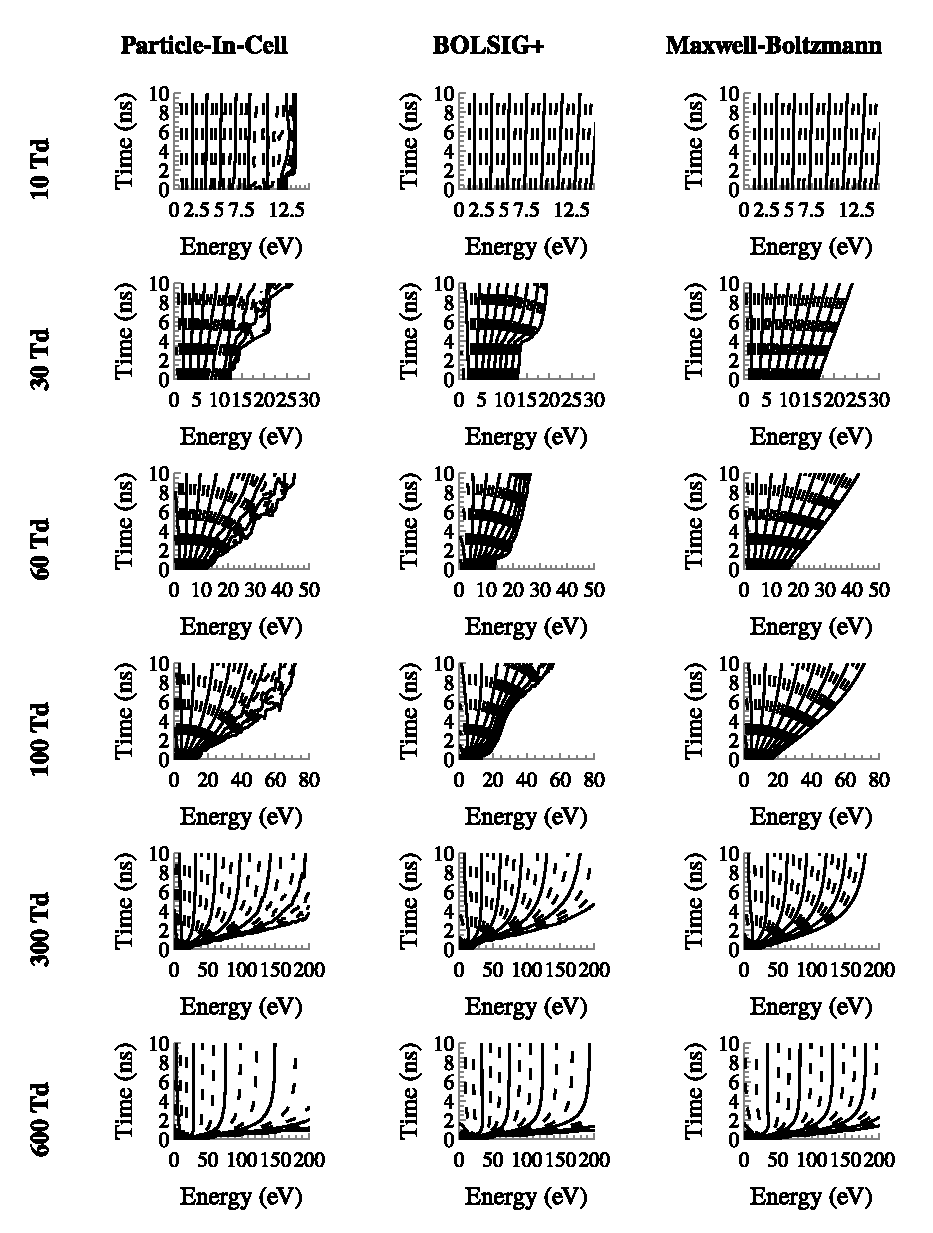
\includegraphics{./chapters/modeling/figures/picmb.eps}
  \caption{Contour plots of the \acs{eedf}s determined from \acs{pic}
    simulations, and the corresponding Maxwell-Boltmzann distributions for a range
    of electric fields.}
  \label{fig:picmb}
\end{figure}
as a series of contour plots. The jaggedness of the \acs{pic} simulations
results from the finite number of particles in the system and the low
probability of high energy electrons. This problem is ameliorated at higher
electric fields where the probability of high-energy electrons increases. It is
also helped by the ionization processes which begin to occur after the first few
nanoseconds.

At 10 Td, the \acs{eedf}s are relatively unchanged over the duration of the
simulation. The subtle slopes of the contours suggest a small increase in the
overall temperature and energy of the system as a function of time. This is more
noticeable at 30 Td, where the contours have a more distinct slope. The spacing
between the slopes is relatively constant for each case--equivalent to a
Maxwell-Boltzmann distribution. However, there is some deviation at low energies
in the case of the BOLSIG+ solutions.

At 60 and 100 Td, the \acs{pic} results begin to exhibit contour spacings which
are consistent at low energies, but begin to grow at higher energies. This is
evidence of a growing population of high-energy electrons, in excess of what
exists in a Maxwell-Boltzmann distribution. Interestingly, the BOLSIG+ solutions
exhibit unique contour shapes which are inconsistent with the other two cases.
Additionally, the spacing of the contours is less consistent, and there is a
dearth of high energy electrons compared to the other cases.

By 300 and 600 Td the situation is reversed, as the Maxwell-Boltzmann
distributions begin to underestimate the population of high energy electrons.
Examination of the individual distributions shows that the \acs{pic} \acs{eedf}s
have a larger population of low energy (less than 20 eV) and high energy
(greater than 100 eV) electrons. This can be explained by the general shape of
the cross sections. The only reactions available to electrons in the \acs{pic}
simulations are elastic scattering, excitation (19.6 eV threshold), and
ionization (24.6 eV threshold). As the inelastic processes turn on at energies
in excess of the 20 eV, the electron population begins to be depleted. Likewise,
the electron population begins to rebound at higher energies as the cross
sections fall off.

Unlike Starikovskaia and Starikovskii's results \cite{Starikovskaia2001} the
various approaches produce comparable \acs{eedf}s. Generally, the
Maxwell-Boltzmann results provide the best match to the \acs{pic} simulations at
electric fields of 100 Td and below. Conversely, the BOLSIG+ results better
represent the \acs{eedf} past 100 eV at the higher field values. That said,
these electrons do not provide a large contribution to the excited states of the
plasma. They are well past the excitation and ionization cross section peaks and
are relatively few in number. Given the larger computational burden of the
Boltzmann solver and the small perceived benefit, it was concluded that the that
the Maxwell-Boltzmann distributions provided an adequate representation of
the \acs{eedf} for the global model.

\subsection{Energy Equation}

The \acs{eedf} provides a means by which to calculate the rate coefficients in
equation~\ref{eq:gcont}. However, as was seen in figure~\ref{fig:picmb}, the
distribution function changes over time. Previously, the \acs{pic} simulations
were used to calculate the time evolution of the mean electron energy, but an
alternate approach was required for the global model.

With suitable assumptions, equation~\ref{eq:energy} (the second moment of the
Boltzmann equation) can provide the means to evolve the mean energy with each
time step. Given the assumptions underlying the global model, the spatial
derivatives can be neglected such that
\begin{equation}
  \frac{d}{dt}\left(\frac{3}{2}p_e\right) =
  \frac{d}{dt}\left(\frac{3}{2}p_e\right)\bigg|_\mathrm{coll}.
\end{equation}
Using the isothermal equation of state \cite{Lieberman2005}, $p=n\kB T$, this
can be rewritten as,
\begin{equation}
  \frac{d}{dt}\left(\frac{3}{2}n_e\kB T_e \right) =
  \frac{d}{dt}\left(\frac{3}{2}n_e\kB T_e \right)\bigg|_\mathrm{coll}.
  \label{eq:energy2}
\end{equation}
The term on the RHS is the collision operator which expresses energy gained or
lost by electrons\footnote{In some plasmas, it is desirable to also treat gas
heating with a similar equation as it can have an appreciable impact on certain
rate constants. However, as noted in Chapter~\ref{chp:metastables}, the gas
temperature of the \acs{rpdn} in question remains at room temperature.} in
particle collisions.

Several different types of energy transfer were considered by the global model.
The first was the heating caused by the electric field. This was followed by
electron energy losses as a result of elastic scattering by the atoms. Finally,
inelastic collisions with all helium states through $n=4$ were considered.
Together, these phenomena replace the term on the RHS of
equation~\ref{eq:energy2} with,
\begin{equation}
  \frac{e^2n_eE(t)^2}{m_ek_m(T_e)N_g}
  - n_ek_m(T_e)N_g\left(\frac{3m_e}{M}\right)\frac{3}{2}\kB(T_e-T_g)
  - n_e \sum_i \sum_{j\neq i} K^e_{ij}N_i\Delta\epsilon_{ij},
  \label{eq:energyparts}
\end{equation}
where $E(t)$ is the time-varying electric field, $k_m$ is the electron momentum
transfer frequency from Pack et al. \cite{Pack1992}, and $\Delta\epsilon_{ij}$
is the energy lost or gained by the electron in atomic (de)excitation reactions.
The first term includes the DC conductivity \cite{Lieberman2005} of the plasma,
and accounts for the heating of the electrons by the electric field. The second
term is the elastic cooling of the electrons by the neutral atoms, where the gas
temperature. The third term is the energy gained or lost by the electrons in
atomic (de)excitation reactions. The
equations~\ref{eq:energyparts},~\ref{eq:energy2} and~\ref{eq:gcont} form the
main components of the global model. Together they provide the means to solve
for the evolution of the electron temperatures, electron densities, excited
state densities, and plasma emissions as functions of time.

\subsection{Model Solutions}

For the purposes of computation, equation~\ref{eq:gcont} can be rewritten for
each atomic state, $i$, resulting in a set of linear, first order differential
equations,
\begin{multline}
  \frac{d}{dt}
  \begin{pmatrix}
    N_1 \\
    N_2 \\
    \vdots \\
    N_M
  \end{pmatrix}
  = n_e
  \begin{pmatrix}
    -\sum_{j\neq 1}K^e_{1,j} & K^e_{2,1}      & \hdots & K^e_{M,1} \\
    K^e_{1,2}      & -\sum_{j\neq 2}K^e_{2,j} & \hdots & K^e_{M,2} \\
    \vdots         & \vdots         & \ddots & \vdots    \\
    K^e_{1,M}      & K^e_{2,M}      & \hdots & -\sum_{j\neq M}K^e_{M,j}
  \end{pmatrix}
  \cdot
  \begin{pmatrix}
    N_1 \\
    N_2 \\
    \vdots \\
    N_M
  \end{pmatrix} \\
  +
  \begin{pmatrix}
    0      & K^o_{2,1}              & \hdots & K^o_{M,1} \\
    0      & -\sum_{j < 2}K^e_{2,j} & \hdots & K^o_{M,2} \\
    \vdots & \vdots                 & \ddots & \vdots    \\
    0      & 0                      & \hdots & -\sum_{j < M}K^e_{M,j}
  \end{pmatrix}
  \cdot
  \begin{pmatrix}
    N_1 \\
    N_2 \\
    \vdots \\
    N_M
  \end{pmatrix} \\
  + N_g
  \begin{pmatrix}
    -\sum_{j\neq 1}K^a_{1,j} & K^a_{2,1}      & \hdots & K^a_{M,1} \\
    K^a_{1,2}      & -\sum_{j\neq 2}K^a_{2,j} & \hdots & K^a_{M,2} \\
    \vdots         & \vdots         & \ddots & \vdots    \\
    K^a_{1,M}      & K^a_{2,M}      & \hdots & -\sum_{j\neq M}K^a_{M,j}
  \end{pmatrix}
  \cdot
  \begin{pmatrix}
    N_1 \\
    N_2 \\
    \vdots \\
    N_M
  \end{pmatrix}, \\
\end{multline}
where $M$ is the total number of atomic states and $\epsilon_i <
\epsilon_{i+1}$. An additional equation can be added to separately account for
electrons as well as electron-specific processes, however the global model used
here assumed quasineutrality by enforcing the relation $N_\mathrm{ion}=n_e$.
Changes in the density of each atomic state were calculated by numerical
integration of these equations. The range of time scales exhibited by the
\acs{rpnd} made it desirable to implement adaptive control of the time step
size. For this reason, the Runge-Kutta-Fehlberg method, adapted from Bradie
\cite{Bradie2006}, was used as the integration scheme.

Initial metastable densities were determined from the \acs{las} measurements and
initial electron densities were determined from \acs{lcif} measurements made by
Weatherford \cite{Weatherford2012a}. However, the \acs{lcif} electron density
measurements were only available for 1.0, 4.0, and 8.0 Torr. Therefore,
subsequent analyses only consider these conditions. Sensitivity to changes in
the initial electron density will be addressed in the following section.

No measurements of the electron temperature in the pre-pulse period were
available. Therefore, it was necessary to assume an electron temperature. Given
the relatively long period of time between pulses, an in initial temperature of
0.2 eV was used. Exploratory simulations found that changes in the initial
electron temperature had a negligible impact on the final distribution of
excited states. Initial excited state densities (not including ions and
metastables) were determined by their values in equilibrium with the 0.2 eV
electrons. Per the results from Chapter~\ref{chp:metastables}, the neutral gas
temperature was fixed at 300 K for the duration of the simulation.

Despite access to the waveform of the applied potential, the actual
time-evolution of the electric field at the metastable measurement points is not
well known. This is a result of the distinctly nonlinear impedance of the
\acs{rpnd} plasma. Takashima et al.\ performed measurements of the electric
field in a \acs{fiw} using a capacitive probe and found it to be significantly
different from the vacuum field. Separately, Ito et al. \cite{Ito2010} and
M\"{u}ller et al. \cite{Muller2011a}, measured the electric fields in a
\acs{rpnd} with a 1.2 mm gap between parallel electrodes using a wave-mixing
approach. They too found a large difference between the vacuum field and the
actual field.

In all three cases, the evolution of the electric field could be best described
by a Gaussian-like pulse, followed by a small, persistent electric field. This
persistent field was on the order of 20-25\% of the peak field value, and would
remain for at least several tens of nanoseconds. The total duration and
magnitude of the persistent field varied between studies and some, such as the
work of Anikin et al. \cite{Anikin1998}, did not appear to record it. Given the
uncertainty associated with the nature of this persistent field, the global
model simulations only considered a single Gaussian pulse. The time domain of
the simulations covered 190 ns with the peak of the pulse centered at 40 ns.

\section{Perturbation Study}

The input values for the global model were relatively fixed, with the exception
of the peak electric field and the width of the pulse. It was initially expected
that the pulse-width would be approximately equal to the width of the applied
pulse, 25 ns. The global models were matched to the metastable measurements by
iterative adjustment of the peak electric field and the pulse-width. However,
there was no clear means by which to estimate the error in the global model
calculations.

In order to provide a partial quantization of this error, a preliminary fit of
the 4.0 Torr data was made and used as a benchmark. Subsequent simulations were
run with small perturbations to the peak electric field, pressure, pulse-width,
and initial electron density. In each case, the benchmark value was perturbed by
$\pm10\%$.

The nominal conditions of the simulation are recorded in table~\ref{tbl:nominal}
\begin{table}
  \centering
  \caption{Nominal simulation parameters for the 4.0 Torr operating condition.}
  \begin{tabular}{llll}
    \toprule
    Pressure & Initial Electron    & Pulse      & Peak Electric \\
    (Torr)   & Density (m$^{-3}$)  & width (ns) & Field (Td)\\ 
    \midrule
    4.0      & 5.36$\times10^{13}$ & 40         & 207 \\
    \bottomrule
  \end{tabular}
  \label{tbl:nominal}
\end{table}
and results of these simulations are shown in figure~\ref{fig:perturbed}.
\begin{figure}
  \centering
  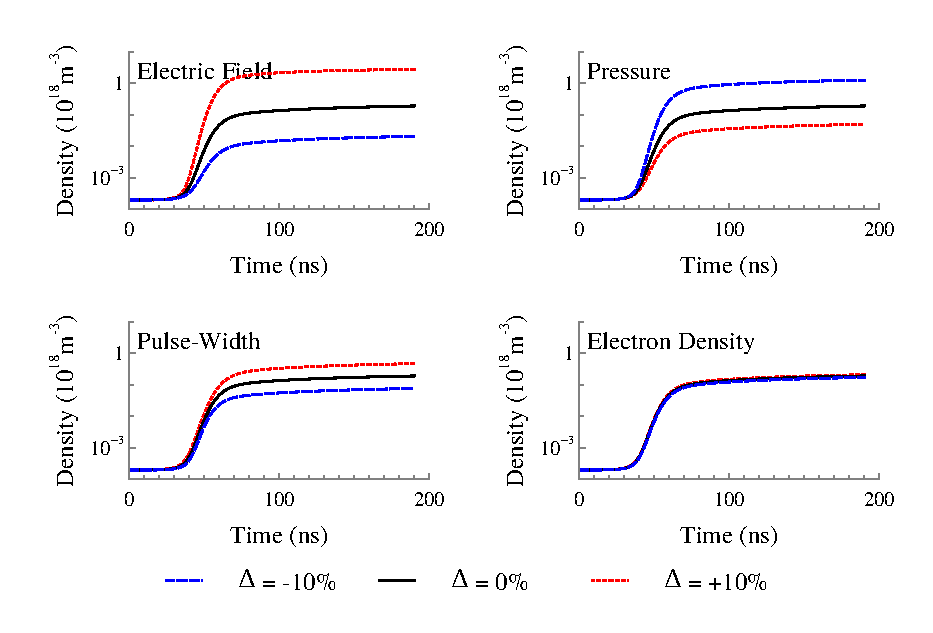
\includegraphics{./chapters/modeling/figures/perturbed.eps}
  \caption{Simulations showing the effects of perturbations to the initial
  conditions on the metastable dynamics.}
  \label{fig:perturbed}
\end{figure}
The metastable trends suggest that the initial electron density has a relatively
small impact on the metastable dynamics. Closer examination reveals that the
final metastable densities change by approximately $\pm10\%$, almost one-to-one
with the initial electron density. In contrast, changes to the pulse-width
produce much more significant changes in the metastable densities. As the
pulse-width is increased, the metastable densities increase. Knowing that the
electric field is fixed, this change can be attributed to the increase in energy
deposited in the electron population.

The two largest factors in the determination of the metastable densities were
the neutral gas pressure and the electric field. The perturbations to these
quantities resulted in largest changes in the final metastable densities. As can
be seen in figure~\ref{fig:perturbed}, increases in pressure corresponded to a
decrease in metastable densities. Changes to the neutral gas pressure tend to
affect the system via several different mechanisms. As seen in
equation~\ref{eq:energyparts}, increases to the gas pressure tend to decrease
the energy deposited in the electrons, and increases losses due to elastic
scattering, thus reducing the energy that can be deposited in excited states.
This competes with the increased number of ground state atoms available for
excitation. That the increase in gas pressure results in a reduced metastable
density indicates that the reduced energy deposition in the electrons is more
important than the increased availability of neutral atoms.

The large impact of the electric field can be traced back to changes in the
ionization rate for each condition. As seen in figure~\ref{fig:ionrates},
\begin{figure}
  \centering
  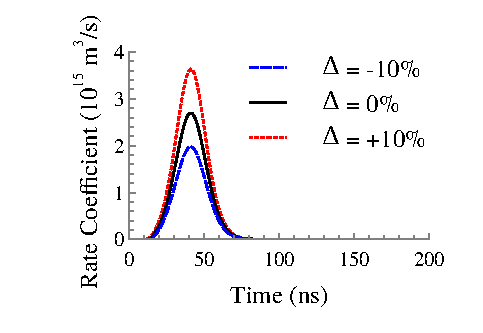
\includegraphics{./chapters/modeling/figures/ionrates.eps}
  \caption{Ionization rates coefficients corresponding to the perturbed electric
  field simulations.}
  \label{fig:ionrates}
\end{figure}
the magnitude of the ionization rate coefficient corresponds to the magnitude of
the electric field. While the changes are somewhat modest, as seen in
Chapter~\ref{chp:theory}, ionization processes exponentially with time. This
means that small changes to the rate coefficient manifest as large differences
in the final electron density. Since the rate of metastable generation is
proportional to the electron density, these changes to the electron density
equate to changes in the metastable density.

\section{Plasma Dynamics}

The plasma dynamics for the 1.0, 4.0, and 8.0 Torr conditions were obtained by
iteratively matching the pulse-width and peak electric field to the metastable
density immediately before the arrival of the reflected pulse. The process was
somewhat complicated by the fact that multiple combinations of the peak field
and pulse-width could produce the same metastable density. Therefore, it was
necessary to fix or otherwise predict one of the values.

Of the two, the pulse-width was the most promising to eliminate as a variable.
The characteristics of the applied pulse already provide reasonable bounds on
the possible widths. Therefore, the 4.0 Torr condition was simulated with a
range of pulse-widths from 5-50 ns with the peak field selected to produce the
same final metastable density in each case. 

The metastable density trend for each pulse-width is compiled in
figure~\ref{fig:widths}.
\begin{figure}
  \centering
  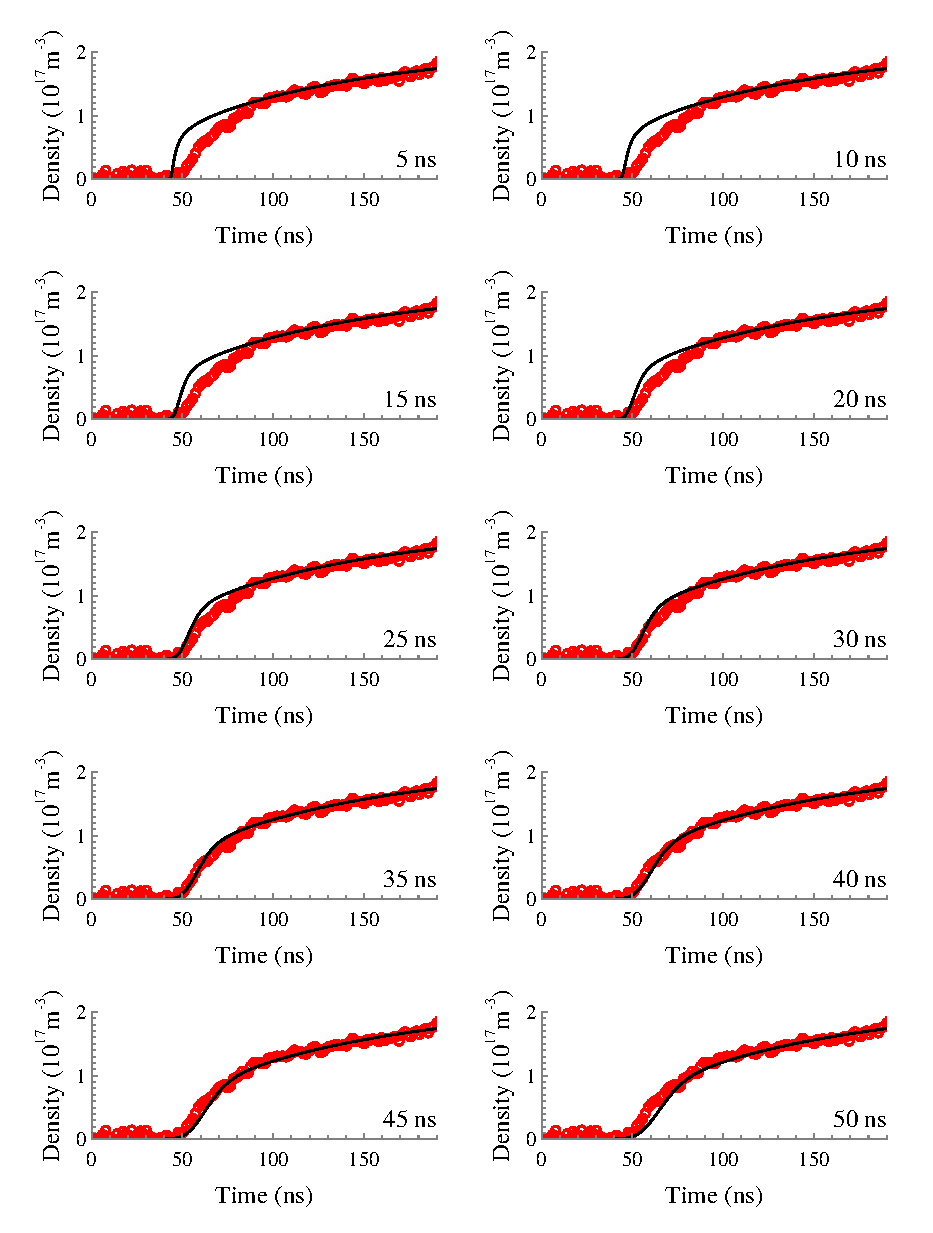
\includegraphics{./chapters/modeling/figures/widths.eps}
  \caption{Effect of the electric field-pulse width on metastable density
  dynamics.}
  \label{fig:widths}
\end{figure}
Several features are immediately apparent. Evident in the plots is a change of
what might be considered the breakdown delay. As the electric field is
increased, observable growth of the metastable density occurs earlier in the
simulation, though the peak electric field remains at the same point in time.
This reflects the faster growth of the electron temperatures during the short
pulse-widths. Increases in the growth rate of the electron temperature allows
the population of electrons to more quickly reach the optimal portions of the
reaction cross sections. Most surprising is the clear need for a pulse-width
that is \emph{longer} than the applied electric field. For the range of
pulse-widths considered, the 40 ns value provides the best match to the measured
metastable data.

The results of the pulse-width comparison suggest that additional excitation is
taking place in addition to the applied pulse. In order to determine the origin
of this excitation, a survey was made of the neutral emissions spectra. The
details of these measurements will be discussed in more detail in
Chapter~\ref{chp:emissions}. The strongest signal was observed at 396 nm,
corresponding to the 4$^1$P$^\mathrm{o}$-2$^1$S transition. Measuring these
emissions as a function of time produced figure~\ref{fig:double}
\begin{figure}
  \centering
  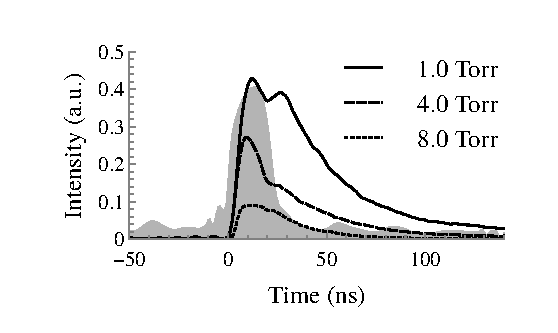
\includegraphics{./chapters/modeling/figures/double.eps}
  \caption{Evidence of return stroke in the double-peaking of plasma emissions.}
  \label{fig:double}
\end{figure}
where the emissions for each operating condition have been overlaid on the
applied voltage pulse. The voltage pulse clearly coincides with an initial
increase in the number of helium atoms in the 4$^1$P$^\mathrm{o}$ state. 15 ns
later, another increase is visible, particularly at 1.0 and 4.0 Torr. This
second transient is similar to the return strokes observed in early streamer
research \cite{Snoddy1936, Loeb1940, Mitchell1947}. The observation of return
strokes in similar, contemporary studies \cite{Vasilyak1994, Pai2009,
Starikovskiy2013} suggests that this is a reasonable explanation for the
double-peaked emissions. If the forward and return stroke possess durations
equal to the applied voltage (25 ns), separated by 15 ns, then the excitation
period would be approximately 40 ns. This is consistent with the pulse-width
required to match the observed data.

Figure~\ref{fig:fieldtau}
\begin{figure}
  \centering
  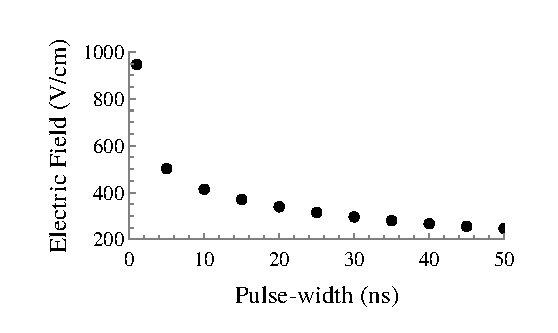
\includegraphics{./chapters/modeling/figures/fieldtau.eps}
  \caption{The required peak field strengths as a function of the pulse-width.}
  \label{fig:fieldtau.eps}
\end{figure}
is a scatter plot of the peak electric fields necessary to obtain the same final
metastable density as a function of the pulse-width. Initially, as the
pulse-width is decreased from 50 ns, only small increases of the electric field
are required to obtain the same number of metastable atoms by the end of the
simulation period. However, as the pulse-width is decreased further, the rate at
which the electric field must increased grows substantially.

Eventually, it is no longer possible to maintain the same metastable density,
despite further increases in the electric field. This occurs for the same reason
that the \acs{eedf} from the \acs{pic} simulations was depressed between 20 and
100 eV--eventually, the cross sections fall off with increasing electron energy.
This places an upper limit on the rate coefficient as a function of electron
temperature. Figure~\ref{fig:longrates}
\begin{figure}
  \centering
  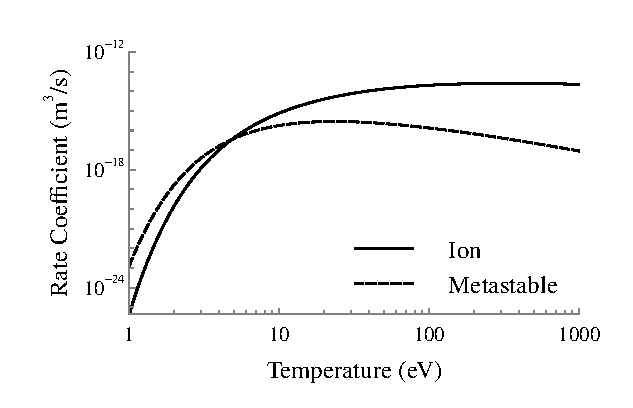
\includegraphics{./chapters/modeling/figures/longrates.eps}
  \caption{Ionization and metastable rate coefficients as functions of
    electron temperature.}
  \label{fig:longrates}
\end{figure}
shows the ionization and metastable rate coefficients as functions of the
electron temperatures in the system. The ionization rate coefficient peaks at
approximately 320 eV, while the metastable rate coefficient peaks much lower at
around 23 eV. These rate coefficients, along with the general form of the cross
sections for the reactions, show that there is an optimal field strength for
ionization and excited state generation. Further increases in the electric field
would only serve to reduce to reduce the final density of these particles.
However, there may still be additional benefits in a higher electric field. The
runaway electrons which can be generated at these field strengths, described by
Vasilyak \cite{Vasilyak1994} among others, could help increase the discharge
volume and homogeneity via nonlocal energy deposition.


\begin{figure}
  \centering
  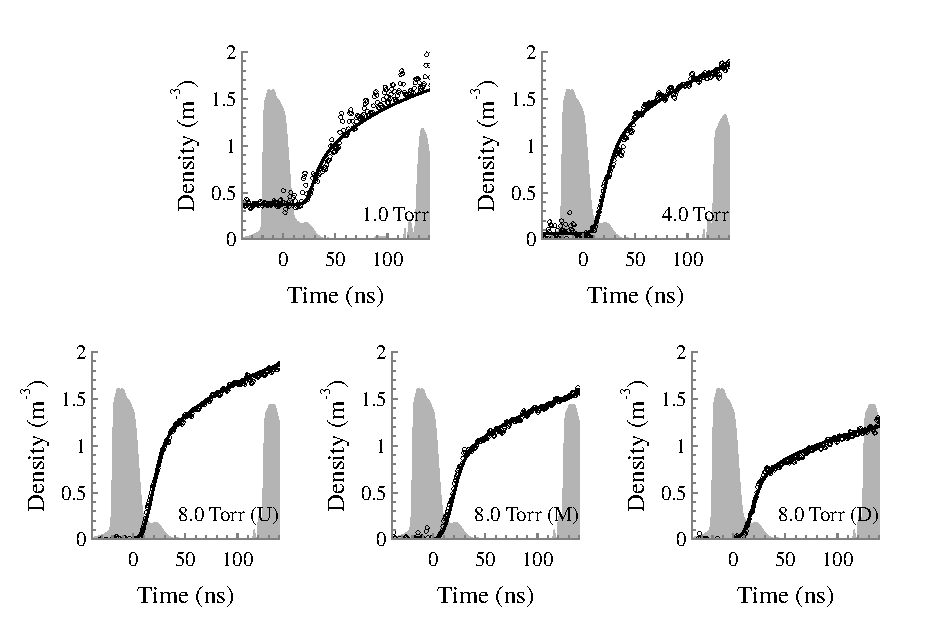
\includegraphics{./chapters/modeling/figures/nmcomp.eps}
  \caption{Comparison of the measured metastable densities to the global model
  simulations.}
  \label{fig:nmcomp}
\end{figure}



\begin{figure}
  \centering
  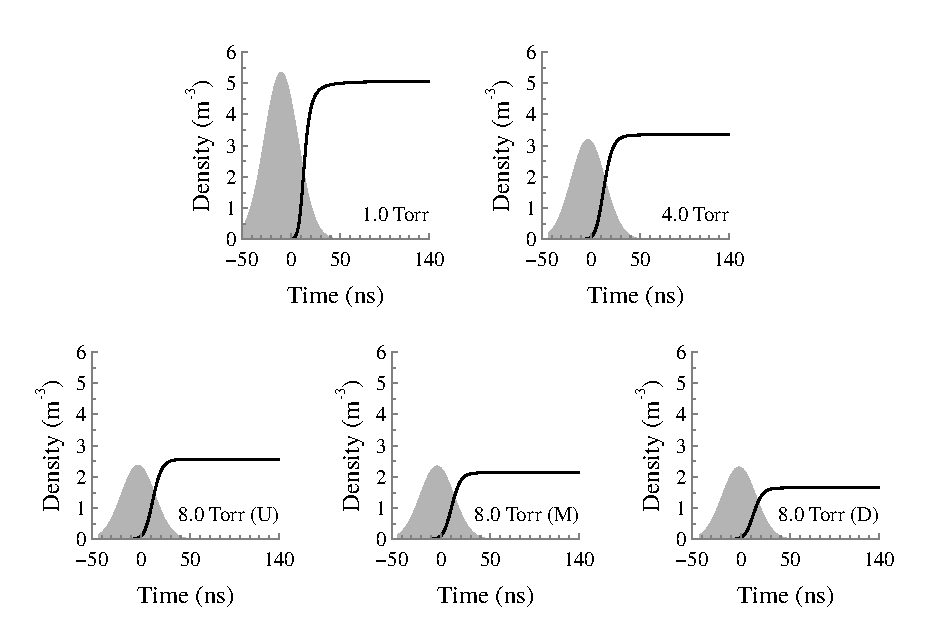
\includegraphics{./chapters/modeling/figures/necomp.eps}
  \caption{Global model predictions of the electrons densities at the simulated
  conditions.}
  \label{fig:necomp}
\end{figure}



\begin{figure}
  \centering
  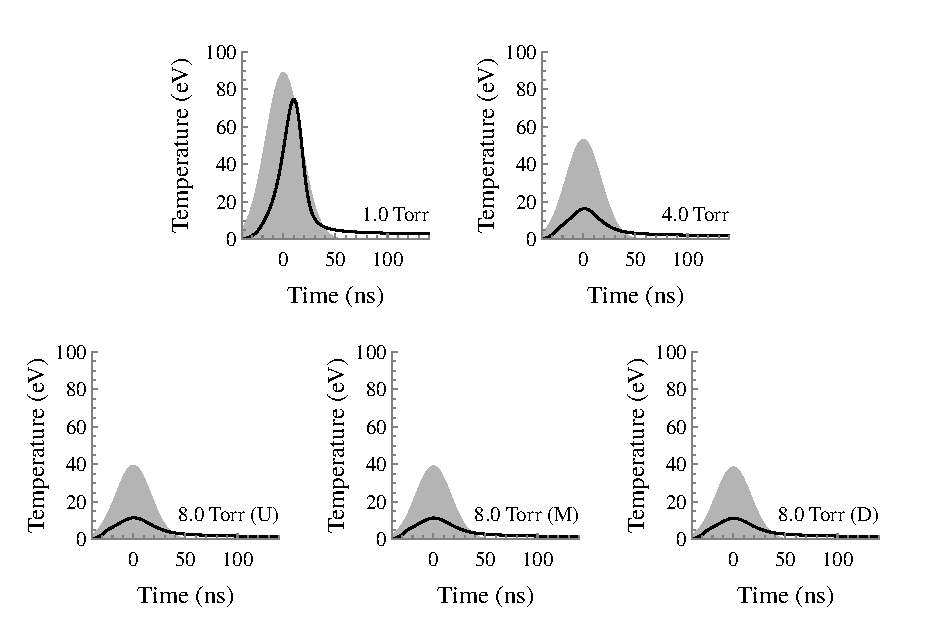
\includegraphics{./chapters/modeling/figures/etemps.eps}
  \caption{Global model predictions of the electron temperatures at the
  simulated conditions.}
  \label{fig:etemps}
\end{figure}



\begin{table}
  \caption{Summary of the peak values for several plasma parameters from the
  global model simulations.}
  \begin{tabular}{lll}
    \toprule \\
    Pressure & E/N  & T$_\mathrm{e}$ & N$_\mathrm{m}$ & n$_\mathrm{e}$ \\
    (Torr)   & (Td) & (eV)           &  (m$^{-3}$)    & (m$^{-3}$) \\
    \midrule \\
    \bottomrule
  \end{tabular}
\end{table}



\section{Summary}


